% !TEX root = /Users/zhuzhuangdi/Desktop/MSUCourses/MachineLearning847/17Project/17spr_wang_zhu_du/Proposal/main.tex
\section{Related Work}  
Approaches to poetry automatic generation can be divided into the following categories.
\begin{description}
\begin{figure*}[t]
	\centering
	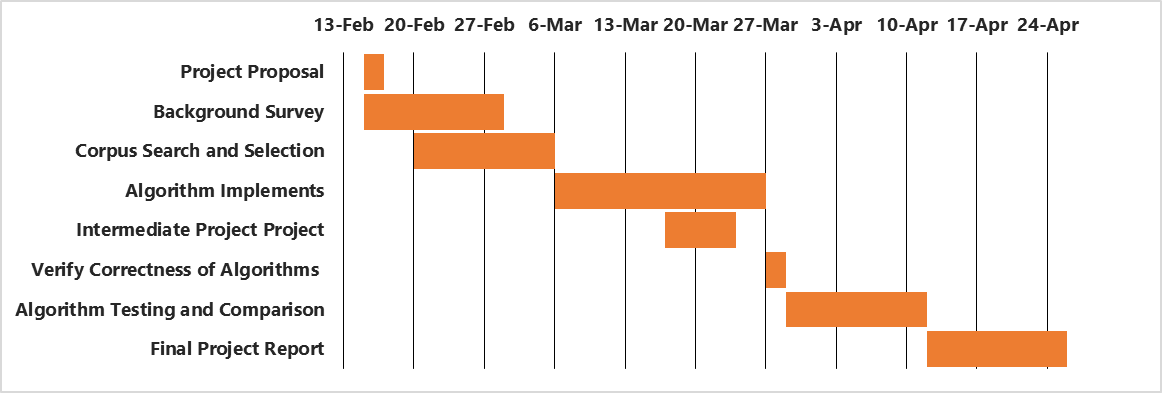
\includegraphics[width=0.8\textheight]
	{ProposedTimeline.png}
	\caption{Time line of project}
	\label{fig:projecttimeline}	
\end{figure*}
\item [Using rules and templates.] 
%
This approach adopts templates to generate poems that comply with grammatical rules, such as the rhythms, lines, and word frequencies\cite{wu2009new,tosa2008hitch}. 
%
However, this approach performs poorly on semantical and poetic requirements.
\item [Using evolutionary algorithms.] This approach is mainly based on evaluation algorithms and search algorithms
%
Natural selection.
\item [Using statistical machine translations (SMT).] 
%Another approach is based on the methods for the generation of other kinds of texts.
\item [Using rankSVM algorithm]
A similar study was conducted on the rap lyrics\cite{malmi2015dopelearning}.  Rap has a formal structure, similar to the Ci we want to research. Feature related to rhyming, structure similarity, and semantic similarity were used fro rankSVM algorithm. The algorithm will try to generate a linear model that can give two lines from a lyrics a relevance score. The score is used to generate the prediction of next line lyrics from a given line of lyrics.
\item [Using neural network.]  This approach adopts an RNN Encoder-Decoder structure \cite{wang2016chinese,bahdanau2014neural}. 
%
They generate new iambics context using previously-generated contexts. The rationale of this approach is that, in Chinese poems, two consecutive lines have high semantical relevance.
\end{description}
